\section{知识图谱可视化展示模块}

\subsection{前端展示设计}

本项目构建了一个面向课程演示和知识浏览的图谱前端页面。页面整体采用左右分栏结构：左侧为知识图谱展示区域，右侧为智能问答区域。用户可以在左侧浏览转座元件相关的局部知识网络，在右侧直接输入自然语言问题并查看回答结果。该设计能够将“图谱展示”和“智能问答”两个模块整合在同一页面中，便于演示和交互。

在数据组织上，图谱页面当前主要围绕 LINE-1 及其相关实体展开，包括：

\begin{itemize}[leftmargin=2em]
  \item TE 节点：例如 LINE-1、L1HS、Alu 等；
  \item Disease 节点：例如阿尔茨海默病、乳腺癌等；
  \item Function 节点：例如逆转录转座、DNA damage 等；
  \item Paper 节点：用于表示支持性文献；
  \item 层级关系边与证据关系边。
\end{itemize}

为了兼顾展示效果和课程答辩使用场景，前端还加入了中英文展示切换。系统在展示层对部分疾病、功能和关系名称做了中英文映射，但底层数据库仍保留较规范的原始命名，以保证检索一致性。

\subsection{核心交互功能}

当前图谱展示模块实现了以下核心交互功能：

\begin{itemize}[leftmargin=2em]
  \item \textbf{节点搜索与定位}：用户可以通过搜索快速定位某个转座元件、疾病或功能节点；
  \item \textbf{节点点击详情}：点击节点后，可在详情区域查看实体类型和关联信息；
  \item \textbf{关系点击查看证据}：点击边后，可查看关系类型及其相关证据描述；
  \item \textbf{图谱布局重排}：页面支持重新布局，使节点在初始展示时尽量分散，减少重叠；
  \item \textbf{局部高亮}：点击节点或边后，可以重点突出局部子图，减轻全图过密导致的阅读困难；
  \item \textbf{中英文切换}：支持面向中文展示和英文展示两种模式。
\end{itemize}

在可视化实现中，项目对布局参数进行了多轮调节，以尽量降低节点和标签重叠问题。特别是对文献节点和证据关系进行了较强的排斥与长度控制，从而让核心 TE、Disease、Function 节点在初始视图中更清晰。

\subsection{图谱页面与后端模块的关系}

该可视化模块并不是孤立页面，而是和图数据库及智能问答系统直接联动：

\begin{itemize}[leftmargin=2em]
  \item 图谱展示使用的是从 Neo4j 组织导出的本地子图数据；
  \item 节点和边的展示逻辑与 Neo4j 中的标签和关系设计保持一致；
  \item 右侧问答面板通过 PHP 后端访问 Neo4j，并将问答结果与图谱页面整合；
  \item 文献节点与关系证据共同支持“可视化展示 + 问答溯源”的完整流程。
\end{itemize}

因此，该模块在整个系统中起到桥梁作用：它既是知识图谱的图形化界面，也是智能问答系统的人机交互入口。

\subsection{网站主要功能截图}

\placeholder{这是 PDF 明确要求的内容。建议至少准备 4 张：图谱首页、节点详情、问答结果、Neo4j 查询结果。}
\begin{figure}[H]
  \centering
  \begin{subfigure}[t]{0.48\linewidth}
    \centering
    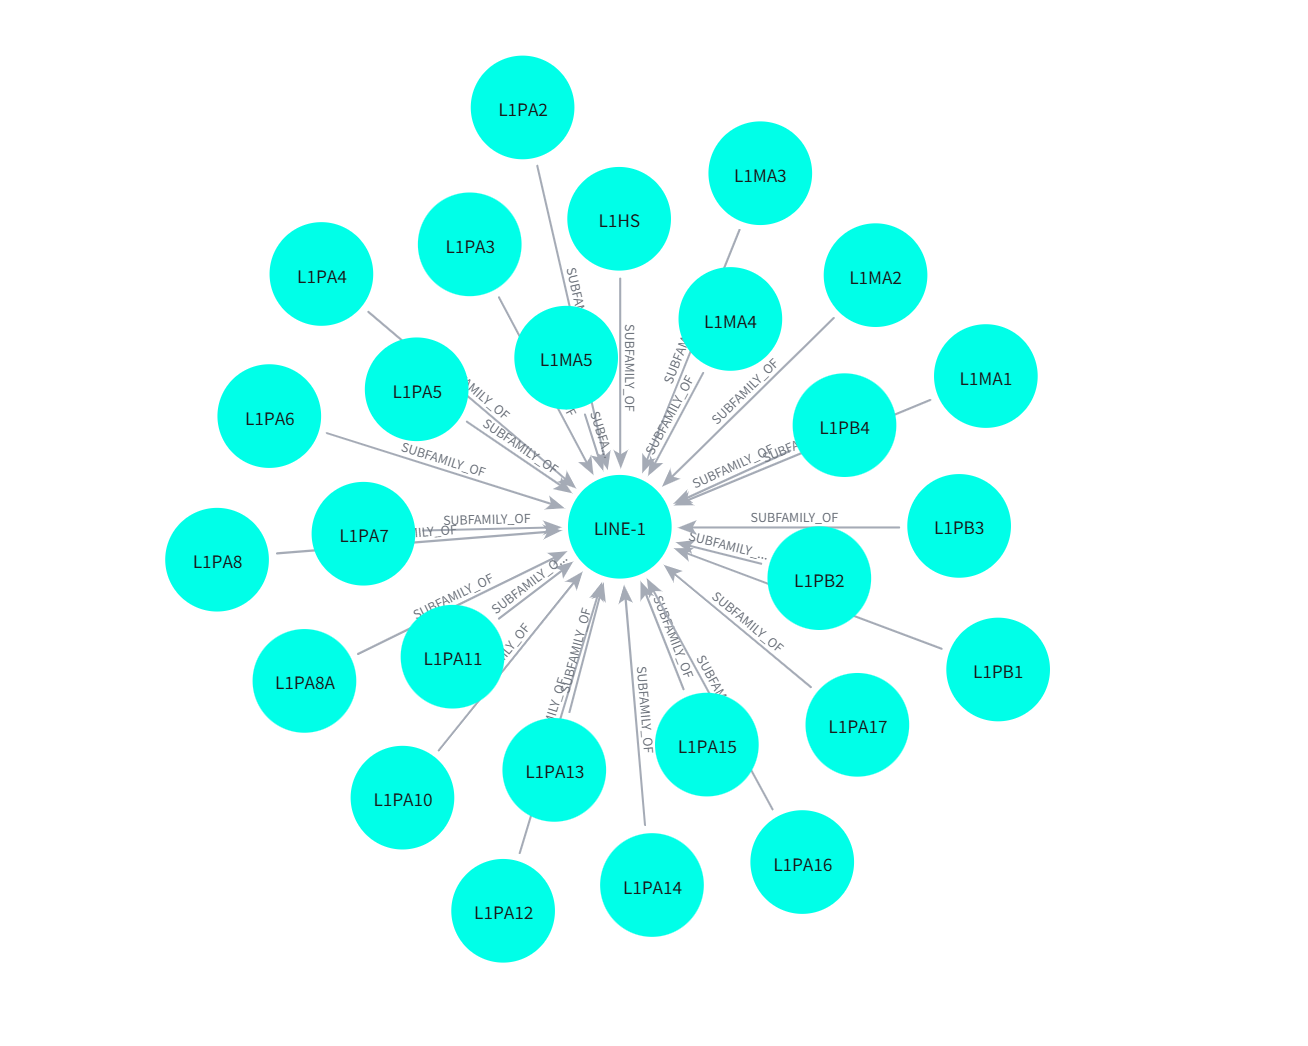
\includegraphics[width=\linewidth]{figures/fig_neo4j_query.png}
    \caption{Neo4j Query 中的 LINE-1 亚家族谱系结果}
    \label{fig:neo4j-query}
  \end{subfigure}
  \hfill
  \begin{subfigure}[t]{0.48\linewidth}
    \centering
    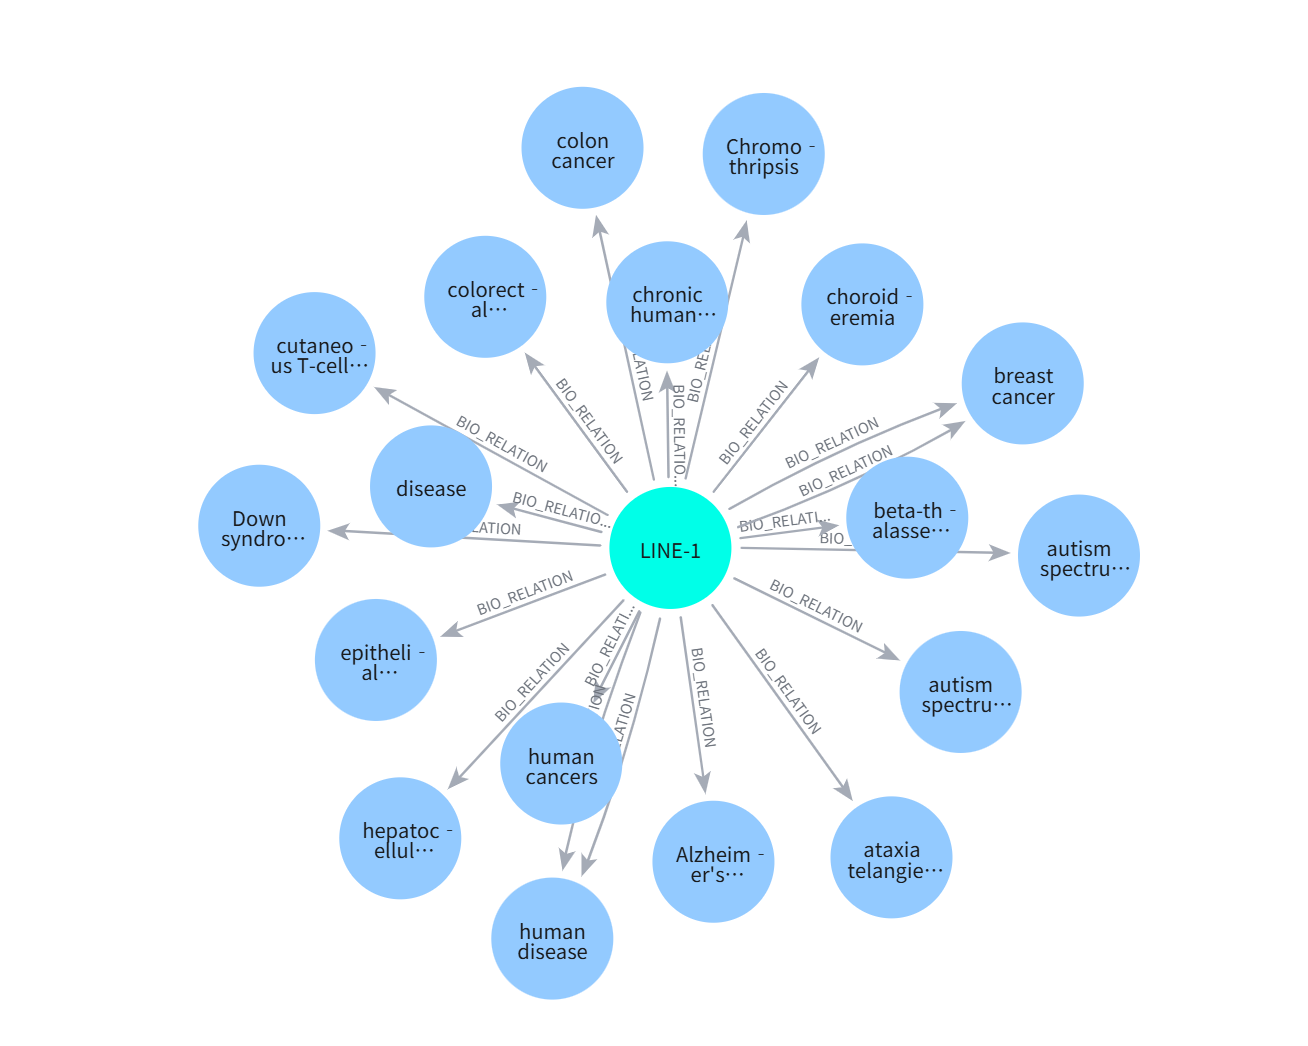
\includegraphics[width=\linewidth]{figures/fig_neo4j_visualisation.png}
    \caption{Neo4j 可视化视图中的局部图谱结构}
    \label{fig:neo4j-visualisation}
  \end{subfigure}
  \caption{图数据库查询结果与可视化展示}
  \label{fig:web-neo4j-pair}
\end{figure}

\figplaceholder{图谱主页截图占位}{fig:web-home}
\figplaceholder{节点详情或关系详情截图占位}{fig:web-detail}
\figplaceholder{问答系统截图占位}{fig:web-qa}
